\documentclass[conference]{IEEEtran}



% *** GRAPHICS RELATED PACKAGES ***
%
\ifCLASSINFOpdf
  % \usepackage[pdftex]{graphicx}
  % declare the path(s) where your graphic files are
  % \graphicspath{{../pdf/}{../jpeg/}}
  % and their extensions so you won't have to specify these with
  % every instance of \includegraphics
  % \DeclareGraphicsExtensions{.pdf,.jpeg,.png}
\else
  % or other class option (dvipsone, dvipdf, if not using dvips). graphicx
  % will default to the driver specified in the system graphics.cfg if no
  % driver is specified.
  % \usepackage[dvips]{graphicx}
  % declare the path(s) where your graphic files are
  % \graphicspath{{../eps/}}
  % and their extensions so you won't have to specify these with
  % every instance of \includegraphics
  % \DeclareGraphicsExtensions{.eps}
\fi
% graphicx was written by David Carlisle and Sebastian Rahtz. It is
% required if you want graphics, photos, etc. graphicx.sty is already
% installed on most LaTeX systems. The latest version and documentation
% can be obtained at: 
% http://www.ctan.org/pkg/graphicx
% Another good source of documentation is "Using Imported Graphics in
% LaTeX2e" by Keith Reckdahl which can be found at:
% http://www.ctan.org/pkg/epslatex
%
% latex, and pdflatex in dvi mode, support graphics in encapsulated
% postscript (.eps) format. pdflatex in pdf mode supports graphics
% in .pdf, .jpeg, .png and .mps (metapost) formats. Users should ensure
% that all non-photo figures use a vector format (.eps, .pdf, .mps) and
% not a bitmapped formats (.jpeg, .png). The IEEE frowns on bitmapped formats
% which can result in "jaggedy"/blurry rendering of lines and letters as
% well as large increases in file sizes.
%
% You can find documentation about the pdfTeX application at:
% http://www.tug.org/applications/pdftex





\usepackage{amsmath}


\usepackage[utf8]{inputenc}
\usepackage{url}
\usepackage{hyperref}
\usepackage{graphicx}
% Packages for listings and color for code excerpts
\usepackage{listings}
\usepackage{color}
\definecolor{shadecolor}{rgb}{.9, .9, .9}

% stuff for nice looking JSON
\usepackage{xcolor}

\colorlet{punct}{red!60!black}
\definecolor{background}{HTML}{EEEEEE}
\definecolor{delim}{RGB}{20,105,176}
\colorlet{numb}{magenta!60!black}

\lstdefinelanguage{json}{
    basicstyle=\scriptsize\ttfamily,
    numbers=left,
    numberstyle=\scriptsize,
    stepnumber=1,
    numbersep=8pt,
    showstringspaces=false,
    breaklines=true,
    frame=lines,
    backgroundcolor=\color{background},
    literate=
     *{0}{{{\color{numb}0}}}{1}
      {1}{{{\color{numb}1}}}{1}
      {2}{{{\color{numb}2}}}{1}
      {3}{{{\color{numb}3}}}{1}
      {4}{{{\color{numb}4}}}{1}
      {5}{{{\color{numb}5}}}{1}
      {6}{{{\color{numb}6}}}{1}
      {7}{{{\color{numb}7}}}{1}
      {8}{{{\color{numb}8}}}{1}
      {9}{{{\color{numb}9}}}{1}
      {:}{{{\color{punct}{:}}}}{1}
      {,}{{{\color{punct}{,}}}}{1}
      {\{}{{{\color{delim}{\{}}}}{1}
      {\}}{{{\color{delim}{\}}}}}{1}
      {[}{{{\color{delim}{[}}}}{1}
      {]}{{{\color{delim}{]}}}}{1},
}

\definecolor{javared}{rgb}{0.6,0,0} % for strings
\definecolor{javagreen}{rgb}{0.25,0.5,0.35} % comments
\definecolor{javapurple}{rgb}{0.5,0,0.35} % keywords
\definecolor{javadocblue}{rgb}{0.25,0.35,0.75} % javadoc
 
\lstset{language=Java,
  basicstyle=\scriptsize\ttfamily,
  numbers=left,
  numberstyle=\scriptsize,
  stepnumber=1,
  numbersep=8pt,
  showstringspaces=false,
  breaklines=true,
  frame=lines,
  backgroundcolor=\color{background},
  keywordstyle=\color{javapurple}\bfseries,
  stringstyle=\color{javared},
  commentstyle=\color{javagreen},
  morecomment=[s][\color{javadocblue}]{/**}{*/},
}
                

% acckorrect bad hyphenation here
\hyphenation{op-tical net-works semi-conduc-tor}


\begin{document}
\title{}


% author names and affiliations
% use a multiple column layout for up to three different
% affiliations
\author{}


% make the title area
\maketitle

% As a general rule, do not put math, special symbols or citations
% in the abstract
\begin{abstract}
\end{abstract}

\section{Introduction}

Middlewares in IoT aim to bridge the gap between the data producers and the data consumers. With the rise of the Internet of Things, comes the need for different applications, and different services with different requirements. Each of these applications will ideally want its own middleware and sensor network so that they can be suited perfectly to their needs. In practical terms this is not possible, as it would be a waste of resources. Therefore, applications will need to work with existing sensor networks and will either develop its own middleware, or choose an existing one that better suits their needs. The question then becomes: how to choose the best one for the task at hand? There are a great number~\cite{razzaque_middleware_2016} of available middlewares to choose from, which makes the selection process very time-consuming. A comparison must be made between them to evaluate which is better suited for which task. But then comes the problem of how to make the evaluation, as performance measuring is not trivial, and common ground must exist for the comparison to be valid. Furthermore, since we have a great number of middlewares, ensuring such common ground will not be possible across different experiments, and different researchers. From these difficulties arises the need for such common ground, a platform that enables multiple comparisons across different middlewares in an efficient manner. To solve these issues, we propose a modular architecture from which will stem a unified platform in which the benchmarks can be run. The main benefits of such a platform are twofold: to provide a common ground in which the middlewares can be benchmarked to ensure equal an playing field, and to ease the addition of other subsequent middlewares.  


\section{Related work}


\section{Solution}

\subsection{Modular Architecture}

In order to achieve the aforementioned requirements, we aim to create a modular architecture by factoring the common elements that go in the creation of any benchmarking application. The general plan for our architecture can be seen in~\ref{fig:benchmark_architecture}.

\begin{figure}[htbp!]
  \centering
  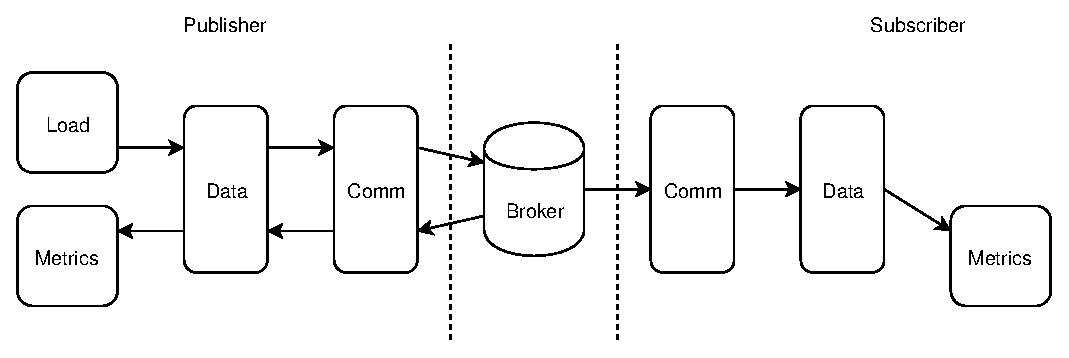
\includegraphics[width=\linewidth]{figures/benchmark_architecture.eps}
  \caption{Main architecture building blocks}
  \label{fig:benchmark_architecture}
\end{figure}

A user must be able to simply swap instances of a block as required. To achieve this, we defined a set of inputs and outputs for each one to maintain modularity. 

The load block will enable different types of IoT scenarios to be programmed and dynamically changed, so that we can attempt to mimic real world scenarios such as Smart Cities. Again, this should be independent from each of the other blocks so that the same workloads can be used throughout all middlewares and protocols, providing a basis for comparison and ensuring high flexibility. 

The data block is where the middleware specific functions reside, and each of these is responsible for implementing its data structure and bridging the gap to the protocols. Similarly to the data block, it is designed so that each is independent so that all can use the same communication methods implemented. With a new middleware entry, one can observe how the existing functions are structured, thereby speeding up the process of implementing its methods. This entry will be added as a new instance of the data block so as to not interfere with the previous middlewares.

Next, we have the communication block where the protocols are lodged, such as HTTP or CoAP, and each has its methods implemented, e.g., POST or GET, so that they are totally platform independent and can be reused. If a new protocol is required to be added to the platform, its methods can be implemented without interfering with the remaining structure.

After the cycle is complete, a set of defined values, such as times and publish request sizes, will be saved and fed into the metrics block, which will extract information from them, such as average publish time or goodput. As we increase the set, more metrics can be generated, without affecting those that are already implemented. 

\subsection{OM2M Implementation}

In an initial phase, we attempted to create an application to benchmark the OM2M middleware with a basis on the work conducted in~\cite{pereira_benchmarking_2018} and \cite{cardoso_benchmarking_2017}, while keeping it as generic as possible to enable future middleware additions and follow our architecture guidelines. This resulted in the structure visible in~\ref{fig:class_diagram_om2m}.

\begin{figure}[htbp!]
  \centering
  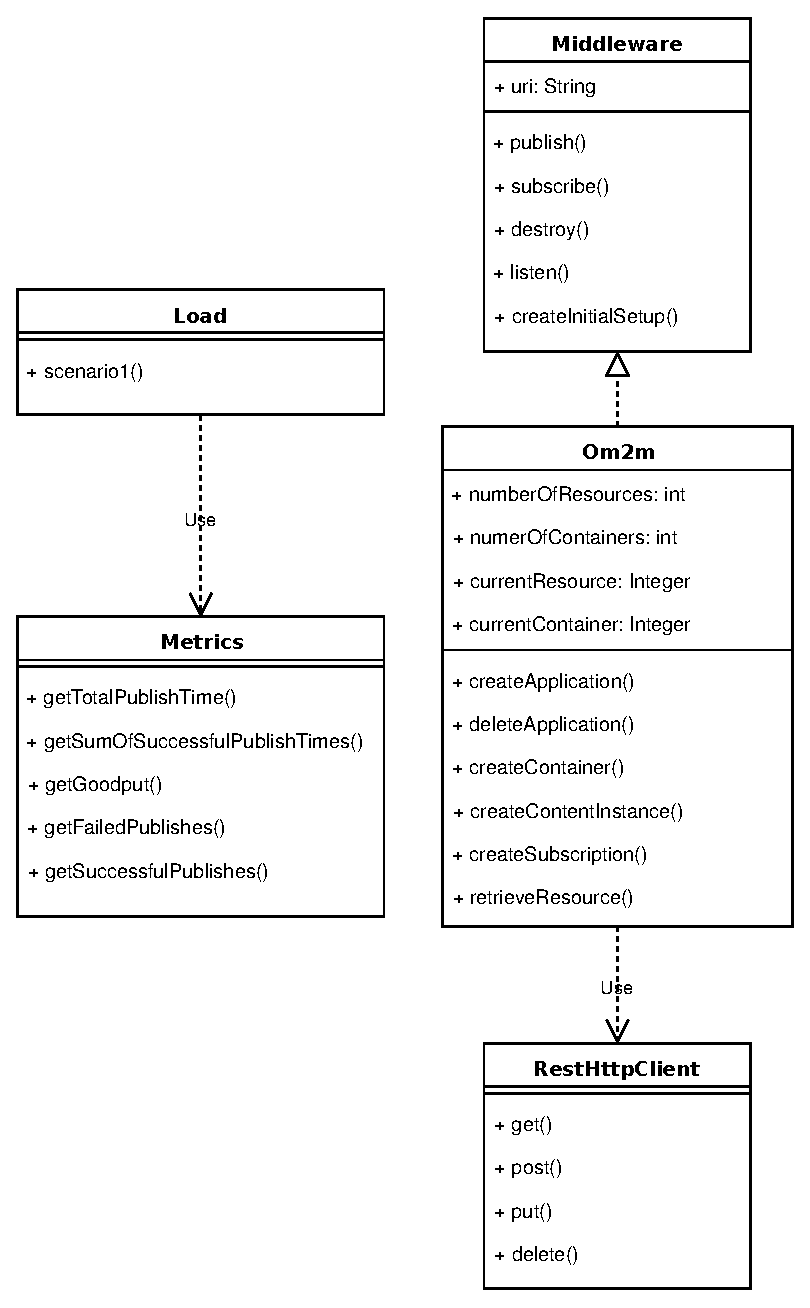
\includegraphics[width=\linewidth]{figures/class_diagram.eps}
  \caption{Class diagram for the initial platform stage}
  \label{fig:class_diagram_om2m}
\end{figure}

Since the load class will be performing the actual requests, it will also call upon the metrics class to perform get the results from the measurements. The load will consist of a certain number of publishes, with a certain message, at a given throughput. All can be easily defined by the user. It's implemented by way of a loop, with each cycle corresponding to a publish request, with sleeps in between to limit the throughput.

\begin{figure}[htbp!]
  \centering
  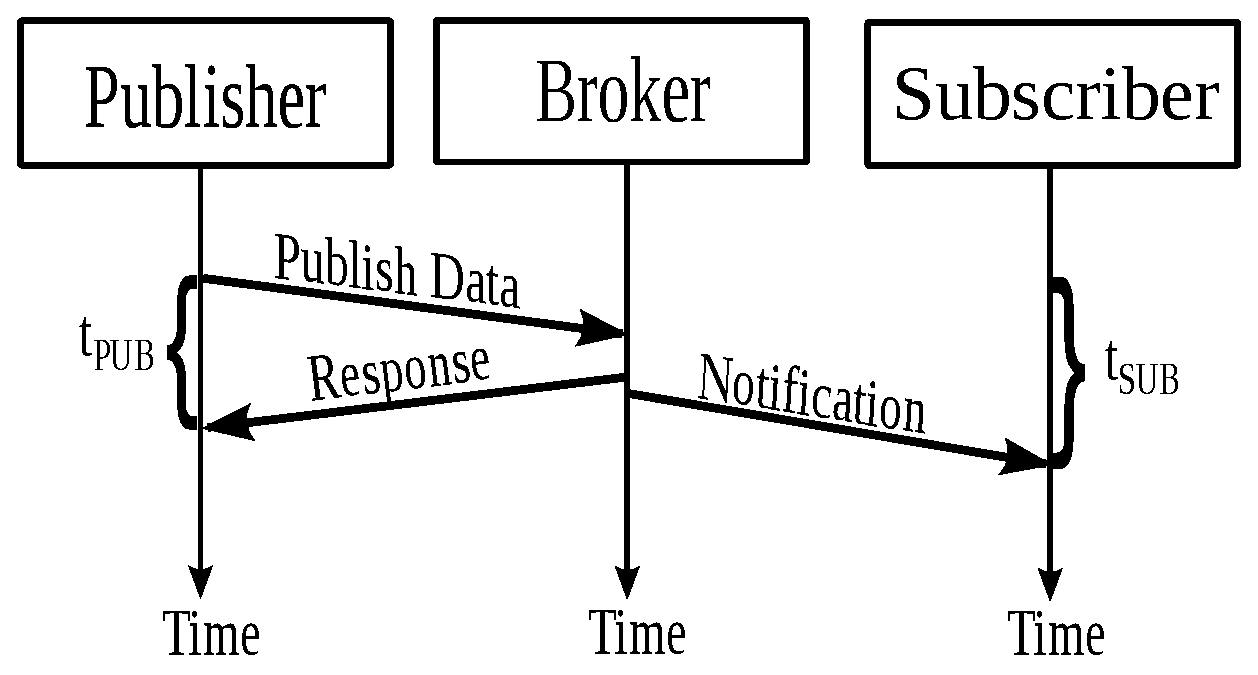
\includegraphics[width=\linewidth]{figures/pub_sub_time.eps}
  \caption{Publish and subscribe times~\cite{cardoso_benchmarking_2017}}
  \label{fig:pub_sub_time}
\end{figure}

The metrics currently implemented on are publish and subscribe time, both visible in~\ref{fig:pub_sub_time}, goodput, failed and successful publishes. Each publish time is simply the difference between sending the request and receiving the response from the broker, easily implemented in the main class by measuring the elapsed time of a single cycle in the load loop.
Goodput is measured by dividing the useful bytes of each message by each publish time. The useful bytes correspond to the full message that is assembled by each middleware. Let's take the Om2m class as an example. Here, a publish request corresponds to the creation of a content instance of the container where we wish to publish. Therefore, the \textbf{createContentInstance()} method will take the message as input and create the appropriate data structure, such as in~\ref{lst:application_creation} for creating an application, to be sent as payload for a certain protocol, e.g., HTTP\@.

\begin{lstlisting}[linewidth=\columnwidth, caption=JSON payload for application creation, captionpos=b, label=lst:application_creation, language=json]
{
   "m2m:ae": {
     "api": "app-sensor",
     "rr": "false",
     "lbl": ["Type/sensor", "Category/temperature", "Location/home"],
     "rn": "MY_SENSOR"
   }
}
\end{lstlisting}

This will be returned to the calling publish method, in order for it to know the payload size for that particular middleware publish request. Since this class extends the \textbf{middleware} superclass, this method is always present and always has the same return values, providing generic metrics.
Following this, we have the failed and successful publishes. In order to determine the whether a certain request was successful or not, some level of analysis must be conducted to the response provided by the broker. Naturally, this is protocol dependent, so in order to create a layer of abstraction, the basic communication methods of the used protocol, such as \textbf{POST} or \textbf{PUT} must return the broker response, in order for the Om2m class to be able to interpret if a publish was successful or not. This way, it will then return to the main class a generic indicator, independent of protocol, indicating its success or failure. 
Lastly, we have subscribe time which is implemented differently, as it potentially relies on times registered at different machines. In order for the subscriber to register the times, a listener must be created for the protocol it is expecting to receive. This listener will be in charge of registering the times at which the notification arrive, meaning this metric is implemented at the protocol level.

Moving on we have the \textbf{Middleware} superclass. Here the goal is to provide the methods that all middlewares are expected to implement and any attributes that are common as well. We therefore chose to have an \textbf{uri} to identify where it will be located on the network. The \textbf{publish()} and \textbf{subscribe()} methods are evident as we are dealing with publish/subscribe scenarios. The \textbf{destroy()} method provides a way to clear any created resources so that the experiment may be conducted again on a clean broker. Next, we have \textbf{listen()}, which is for the subscriber to call so that it may receive and parse notifications as needed, and register their arrival times. Finally, \textbf{createInitialSetup()} is for registering resources, such as applications in the case of OM2M, the number of which is defined by the user.

Then, we come to the protocol classes. Currently, only HTTP is implemented in the \textbf{RestHttpClient()}, but others may be added in the future, such as CoAP or MQTT\@. The four methods are ubiquitous across several applications, and typically most middelwares which rely on HTTP will make use of these. 


\section{Evaluation}

\subsection{Adding new middlewares}

The platform development was always conducted taking into account the addition of new middlewares, therefore it was made to be as generic as possible and to facilitate any new addition. However, during such an addition, there can always be details which were not accounted for and can force the platform to change to be able to accommodate this new addition. In this section, we will see the changes to the architecture, and the differences and similarities between the both implementations, how much was reusable in terms of code and overall structure, and attempt to quantify the changes through the number of lines of code. 

\subsubsection{FIWARE}

We decided to add the FIWARE middleware as a result of previous work and greater familiarity with it. The class diagram is similar to that in figure~\ref{fig:class_diagram_om2m}, with the difference being the new Fiware class, visible in~\ref{fig:class_diagram_fiware}.

\begin{figure}[htbp!]
  \centering
  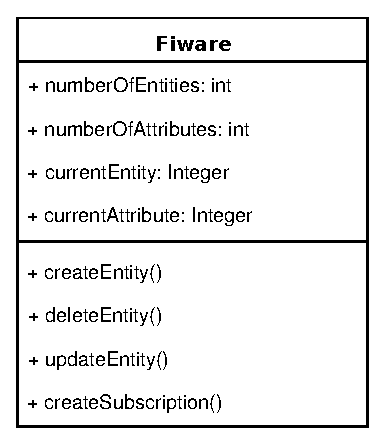
\includegraphics[width=0.5\columnwidth]{figures/class_diagram_fiware.eps}
  \caption{Fiware class diagram}
  \label{fig:class_diagram_fiware}
\end{figure}

Since it is also an extension of the \textbf{Middleware} superclass, it shares the five methods and attributes with \textbf{Om2m}, with the rest being specific the this class, with a similar structure. The superclass methods will call the specific functions to bridge the gap to the communication protocol, in this case HTTP. Starting with \textbf{publish()}, the structure is basically identical, with only 4 lines of code being different between both middlewares out of 22, which merely correspond to differing function calls and variable names. A Om2m publish calls upon the \textbf{createContentInstance()} function to create a new instance in a previously created container in an application, receiving the intended message and constructing a JSON payload in accordance to its standards, and sending it via an HTTP POST. Similarly, Fiware uses the \textbf{updateEntity()} method to update the current status of an entity, also constructing an appropriate JSON, but sending it with an HTTP PATCH. A key detail to note here, is that using this method, Fiware does not retain memory of previous status, as it is overwritten. Both of these methods return the JSON payloads and the HTTP response, and register the times at which the publishes were sent. The \textbf{subscribe()} method in both implementations is similar to this, but Fiware also uses HTTP POST as opposed to a PATCH request.

The \textbf{listen()} function is the same in both, as it only creates an HTTP server for the subscriber to listen and parse the notifications.

Next, we have \textbf{destroy()} which aims to delete all the created resources so that it is easy to start from scratch. For this, Om2m calls \textbf{deleteApplication()} which takes the name of the resource to be deleted, constructs the JSON payload and POSTs it to the broker. For Fiware its \textbf{deleteEntity()}, and it works much the same, the only change being the JSON created.

Finally we have \textbf{createInitialSetup()}, where resources are registered for the first time. For Om2m, a nested \textbf{for} loop is used to create the desired number of applications with \textbf{createApplication()}, and for each of these the number of containers with \textbf{createContainer()}. For Fiware, the number of attributes must be defined upon entity creation, so these are handled on a lower level at the \textbf{createEntity()} method, so only a simple \textbf{for} loop is used to create the necessary entities.

Almost all functions used share the same structure: create the JSON to encapsulate the message, create the appropriate HTTP headers and make the HTTP request to the broker. This greatly eases the process of adding middlewares.

\subsubsection{Ponte}

As before, there is an URI identifier and two variables that indicate how many resources and attributes per resource this middleware instance will take. With Ponte, only the \textbf{publish()} and createInitialSetup methods from the \textbf{Middleware} superclass was implemented. The reason for this is that there was no need to create an additional abstraction layer between the the middleware specific methods and the publish method as before with other implementations, since a simple HTTP PUT is required with the target resource and attribute in the URL, and the value as payload, without any need for JSON or XML assembly.

\textbf{subscribe()} and \textbf{listen()} were not implemented as there is no way for the broker to notify a subscriber through HTTP, only through GETs originating from the subscriber, which would require periodic queries in order to keep the status updated and differs from a publish/subscribe scenario.

There is no obvious way of deleting a resource so \textbf{destroy} is also not implemented, with the most obvious way to do so being simply to restart the broker. 

\subsection{Benchmarking results}

The goal here is not to use the results to evaluate the performance of the platform, or to make a comparison between other middlewares. Rather, we want to use the results to validate the platform itself, and show what types of information we can extract from these tests, while still keeping the platform generic.

The test consisted of 20000 publishes of 15 byte messages, at a rate of 100 publishes per second. In~\ref{fig:publish_times} we can see a comparison between the publish times of all three implemented middlewares. In~\ref{fig:subscribe_times} only FIWARE and OM2M are present, as it is not possible to measure the subscribe times with Ponte using HTTP. 

\begin{figure}[htbp!]
  \centering
  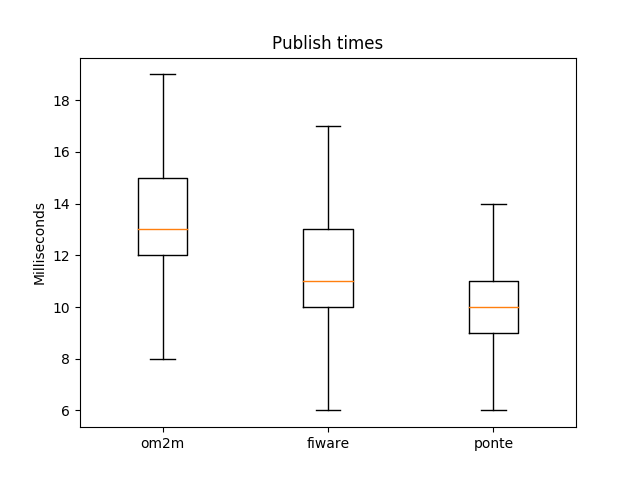
\includegraphics[width=\columnwidth]{figures/om2m_fiware_ponte_publish_times.png}
  \caption{OM2M publish times}
  \label{fig:publish_times}
\end{figure}

\begin{figure}[htbp!]
  \centering
  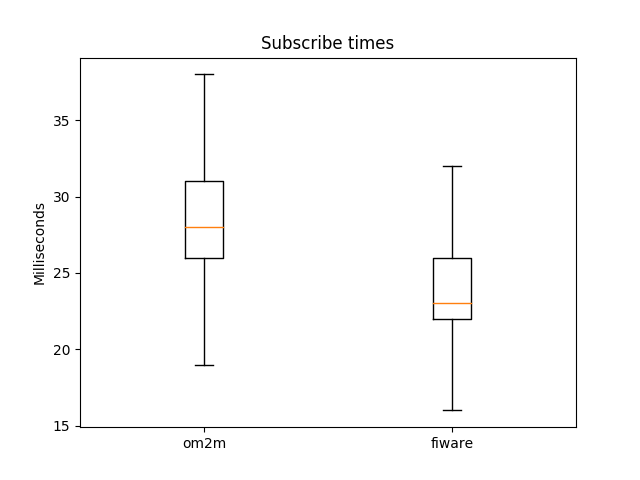
\includegraphics[width=\columnwidth]{figures/om2m_fiware_subscribe_times.png}
  \caption{OM2M subscribe times}
  \label{fig:subscribe_times}
\end{figure}

A few extra metrics are available for each of them, being those the Goodput, total publish time, number of failed and successful publishes.

\subsubsection{FIWARE}
\begin{itemize}
\item Goodput: 3.54 KB/s
\item Failed publishes: 0
\item Successful Publishes: 20000
\item Total publish time: 602 seconds
\end{itemize}

\subsubsection{OM2M}
\begin{itemize}
\item Goodput: 4.15 KB/s
\item Failed publishes: 0
\item Successful Publishes: 20000
\item Total publish time: 655 seconds
\end{itemize}

\subsubsection{Ponte}
\begin{itemize}
\item Goodput: 1.33 KB/s
\item Failed publishes: 0
\item Successful Publishes: 20000
\item Total publish time: 535 seconds
\end{itemize}



\section{Conclusion}



% trigger a \newpage just before the given reference
% number - used to balance the columns on the last page
% adjust value as needed - may need to be readjusted if
% the document is modified later
%\IEEEtriggeratref{8}
% The "triggered" command can be changed if desired:
%\IEEEtriggercmd{\enlargethispage{-5in}}

% references section

% can use a bibliography generated by BibTeX as a .bbl file
% BibTeX documentation can be easily obtained at:
% http://mirror.ctan.org/biblio/bibtex/contrib/doc/
% The IEEEtran BibTeX style support page is at:
% http://www.michaelshell.org/tex/ieeetran/bibtex/
%\bibliographystyle{IEEEtran}
% argument is your BibTeX string definitions and bibliography database(s)
%\bibliography{IEEEabrv,../bib/paper}
%
% <OR> manually copy in the resultant .bbl file
% set second argument of \begin to the number of references
% (used to reserve space for the reference number labels box)

\bibliographystyle{unsrt}
\bibliography{biblio}


% that's all folks
\end{document}


%%% Local Variables:
%%% mode: latex
%%% TeX-master: t
%%% End:

